\documentclass[17pt, t, lualatex]{beamer}

%% ============================================================
%% Master's thesis defence
%% Paul Mayer -- KTH Royal Institute of Technology
%% "Surrogate Gradients for Gradient-Based Parameter Estimation
%%  in Simplified Neuron Models"
%% Theme: kthpq (Isaac Ren), MIT-licensed. See LICENSE.txt.
%% ============================================================

\title{Between Two Worlds}
\subtitle{\large Surrogate Gradients for Gradient-Based Parameter\\Estimation in Simplified Neuron Models}
\date{August 31st, 2026}
\institute[KTH]{KTH Royal Institute of Technology}
\author{Paul Mayer}

\usepackage{amsmath,amssymb,mathtools}
\usepackage{multicol}
\usepackage{hyperref}
\usepackage{booktabs}
\usepackage{dsfont}
\usepackage{pifont}
\usepackage{tikz}
\usetikzlibrary{shapes,arrows,positioning,calc,decorations.pathreplacing,backgrounds}

% Probably load as late as possible
\usetheme[engine=lualatex, mathshape=sf, fontdir=kthpq-files/fonts/Figtree/]{kthpq}
\setmonofont{Bitstream Vera Sans Mono}[Scale=.9]

% Look in the local figures/ folder first, then keep the theme's logo/lines path.
\graphicspath{{figures/}{kthpq-files/figs/}}

% On-brand alert colour (KTH brick) instead of the default beamer red.
\setbeamercolor{alerted text}{fg=dark brick}
\setbeamertemplate{itemize items}[circle]
\setbeamertemplate{caption}{\raggedright\insertcaption\par}

% Convenience colours pulled from the KTH palette (defined in the colour theme).
\newcommand{\good}[1]{{\color{dark green}#1}}
\newcommand{\bad}[1]{{\color{dark brick}#1}}
\newcommand{\hl}[1]{{\color{KTH blue}#1}}
\newcommand{\cmark}{{\color{dark green}\ding{51}}}
\newcommand{\xmark}{{\color{dark brick}\ding{55}}}
% Loss symbol. Fira Math (the sf math font) has no script/calligraphic L
% (U+2112), so we use a plain italic L, which is unambiguous in context.
\newcommand{\Loss}{L}

% A compact "takeaway" strip at the bottom of a content slide.
\newcommand{\takeaway}[1]{%
  \vfill
  {\centering\usebeamercolor[fg]{structure}%
   \small\textbf{#1}\par}%
  \vspace{2pt}%
}

\begin{document}

%% ============================================================
%% TITLE
%% ============================================================
\inserttitlepage

%% ============================================================
%% ROADMAP
%% ============================================================
\begin{frame}{Where we are going}
\begin{columns}[T]
\begin{column}{0.5\textwidth}
\textbf{The big picture} \good{(5 min)}
\begin{itemize}
  \item Why simulate neurons?
  \item Why tuning them is hard
  \item The surrogate-gradient idea
\end{itemize}
\vspace{0.3cm}
\textbf{The contribution}
\begin{itemize}
  \item A differentiable AdEx in \texttt{Jaxley}
  \item Fast \emph{and} trainable
\end{itemize}
\end{column}
\begin{column}{0.5\textwidth}
\textbf{The core question}
\begin{itemize}
  \item Which loss can a gradient descend?
  \item Does gradient fitting actually work?
\end{itemize}
\vspace{0.3cm}
\textbf{The honest answer}
\begin{itemize}
  \item A systematic benchmark
  \item \bad{Where it fails} --- and \good{where it does not}
\end{itemize}
\end{column}
\end{columns}
\takeaway{A story of two worlds: gradient-based optimization and simplified spiking neurons.}
\end{frame}

%% ============================================================
%% PART I -- THE BIG PICTURE (general audience)
%% ============================================================
\section{The Big Picture}
\insertsectionpage

%% ---- SLIDE: The dream ----
\begin{frame}{The dream: simulating the brain}
\begin{center}
\begin{tikzpicture}[
    box/.style={draw, rounded corners=8pt, minimum width=3.2cm, minimum height=1.6cm,
                align=center, font=\normalsize, thick},
    arrow/.style={->, very thick, >=stealth}
]
    \node[box, fill=light brick] (brain) at (0,0) {
        \LARGE\strut Brain\\[3pt]
        \small 86 billion neurons
    };
    \node[box, fill=light yellow] (detail) at (7,1.8) {
        Detailed models\\[3pt]
        \small accurate but slow
    };
    \node[box, fill=light green] (simple) at (7,-1.8) {
        Simplified models\\[3pt]
        \small fast, but tuning breaks
    };
    \node[box, fill=light blue] (sim) at (16,0) {
        \LARGE\strut Simulation\\[3pt]
        \small understand disease,\\[-2pt]
        \small develop treatments
    };
    \draw[arrow, brick, dashed] (brain) -- (detail);
    \draw[arrow, dark green] (brain) -- (simple);
    \draw[arrow, brick, dashed] (detail) -- node[above, sloped, font=\small, text=brick] {too expensive} (sim);
    \draw[arrow, dark green, line width=2pt] (simple) -- node[below, sloped, font=\small, text=dark green] {feasible} (sim);
\end{tikzpicture}
\end{center}
\takeaway{Simplified models make large-scale brain simulation possible --- but they must be \alert{tuned} to match real neurons.}
\end{frame}

%% ---- SLIDE: The tuning problem ----
\begin{frame}{Tuning a neuron model}
\begin{center}
\begin{tikzpicture}[
    box/.style={draw, rounded corners=6pt, minimum width=2.8cm, minimum height=1.3cm,
                align=center, font=\normalsize, thick}
]
    \begin{scope}[xshift=-4cm, yshift=1cm]
        \node[box, fill=light blue] (real) at (0,2.2) {Real neuron\\recording};
        \node[box, fill=light yellow] (model) at (0,-1) {Neuron model};
    \end{scope}
    \begin{scope}[xshift=4cm, yshift=0cm]
    \draw[thick, gray] (-3.2,-2.8) -- (3.2,-2.8);
    \foreach \x/\lab in {-2.5/leak, -0.8/reset, 0.8/adapt, 2.5/slope} {
        \draw[thick, fill=white] (\x,-2.8) circle (0.35);
        \draw[thick, rotate around={30:(\x,-2.8)}] (\x,-2.8) -- ++(0,0.35);
        \node[font=\tiny, below] at (\x,-3.25) {\lab};
    }
    \node[font=\small, left] at (-3.5,-2.8) {Parameters:};
    \end{scope}
    \begin{scope}[xshift=0cm, yshift=2.2cm]
        \draw[->] (0,0) -- (4.5,0) node[right, font=\small] {time};
        \draw[->] (0,-0.3) -- (0,1.8);
        \draw[KTH blue, thick] (0.2,0.4) -- (0.8,0.5) -- (1,1.5) -- (1,0.3) -- (2,0.4) -- (2.2,1.5) -- (2.2,0.3) -- (3.3,0.4) -- (3.5,1.5) -- (3.5,0.3) -- (4.2,0.4);
        \node[KTH blue, font=\small, right] at (4.5,1.2) {real};
    \end{scope}
    \begin{scope}[xshift=0cm, yshift=-1cm]
        \draw[->] (0,0) -- (4.5,0) node[right, font=\small] {time};
        \draw[->] (0,-0.3) -- (0,1.8);
        \draw[brick, thick, dashed] (0.2,0.4) -- (1.0,0.5) -- (1.2,1.5) -- (1.2,0.3) -- (2.5,0.5) -- (2.7,1.5) -- (2.7,0.3) -- (4.2,0.5);
        \node[brick, font=\small, right] at (4.5,1.2) {model};
    \end{scope}
    \draw[->, thick] (real) -- ++(3.5,0);
    \draw[->, thick] (model) -- ++(3.5,0);
    \node[font=\Large, dark yellow] at (8.5,1.4) {\textbf{Match?}};
    \draw[->, very thick, dark yellow, dashed] (8.5,0.8) -- (8.5, 0.4) node[below, font=\small, text=black] {adjust knobs};
    \draw[->, thick, dark yellow, dashed] (8.5, -0.5) -- (6.5,-2.2);
\end{tikzpicture}
\end{center}
\takeaway{\textbf{Goal:} automatically find the parameter settings that reproduce the recording.}
\end{frame}

%% ---- SLIDE: The obstacle ----
\begin{frame}{The obstacle: spikes break the math}
\begin{columns}[c]
\begin{column}{0.52\textwidth}
\begin{center}
\begin{tikzpicture}[scale=1.0]
    \draw[->] (0,0) -- (6,0) node[right, font=\small] {time};
    \draw[->] (0,-0.5) -- (0,4) node[above, font=\small] {voltage};
    \draw[KTH blue, very thick] (0.3,1) -- (1.5,1.2) -- (2.5,1.5);
    \draw[KTH blue, very thick] (2.5,1.5) -- (2.8,3.5);
    \draw[dashed, gray] (0,2.5) -- (6,2.5);
    \node[gray, font=\small, right] at (6,2.5) {threshold};
    \draw[brick, ultra thick] (2.8,3.5) -- (2.8,0.5);
    \node[brick, font=\small, right] at (3.2,2.0) {\textbf{RESET}};
    \node[brick, font=\small, right] at (3.2,1.3) {(the cliff)};
    \draw[KTH blue, very thick] (2.8,0.5) -- (4,0.8) -- (5.5,1.1);
    \draw[<-, thick, brick] (2.9,3.2) -- (4.5,4.5) node[right, font=\small, text=black, align=left] {Gradient tuning\\needs smooth\\curves};
\end{tikzpicture}
\end{center}
\end{column}
\begin{column}{0.45\textwidth}
\begin{center}
\begin{tikzpicture}[scale=1.1]
    \draw[->] (-1.8,0) -- (2,0);
    \draw[->] (0,-0.3) -- (0,2.2);
    \draw[KTH blue, ultra thick] (-1.5,0) -- (0,0);
    \draw[KTH blue, ultra thick] (0,1.5) -- (1.5,1.5);
    \draw[KTH blue, fill=white, thick] (0,0) circle (0.07);
    \draw[KTH blue, fill=KTH blue] (0,1.5) circle (0.07);
    \node[font=\small, below] at (0,-0.5) {spike threshold};
    \node[font=\normalsize, above, align=center] at (0,2.3) {Spike function};
    \node[brick, font=\small, align=center] at (0,-1.7) {Slope $=0$ everywhere\\$\Rightarrow$ no gradient signal!};
\end{tikzpicture}
\end{center}
\end{column}
\end{columns}
\takeaway{Gradient tuning is fast --- but the spike is a \alert{cliff} that blocks the gradient.}
\end{frame}

%% ---- SLIDE: The trick ----
\begin{frame}{The trick: surrogate gradients}
\begin{columns}[c]
\begin{column}{0.44\textwidth}
\begin{center}
\begin{tikzpicture}[
    box/.style={draw, rounded corners=6pt, minimum width=3cm, minimum height=1cm,
                align=center, font=\normalsize, thick}
]
    \node[box, fill=light blue] (fwd) at (0,2) {Simulation\\(forward)};
    \node[box, fill=light green] (bwd) at (0,-1) {Tuning\\(backward)};
    \node[font=\small, right, align=left] at (2.1,2) {real spike};
    \node[font=\small, right, align=left] at (2.1,-1) {smooth\\ stand-in};
    \begin{scope}[xshift=6.6cm, yshift=1.7cm, scale=0.7]
        \draw[->] (-1.2,0) -- (1.2,0);
        \draw[->] (0,-0.2) -- (0,1.5);
        \draw[KTH blue, very thick] (-1,0) -- (0,0);
        \draw[KTH blue, very thick] (0,1) -- (1,1);
    \end{scope}
    \begin{scope}[xshift=6.6cm, yshift=-1.3cm, scale=0.7]
        \draw[->] (-1.2,0) -- (1.2,0);
        \draw[->] (0,-0.2) -- (0,1.5);
        \draw[dark green, very thick]
            (-1,0.01) -- (-0.6,0.05) -- (-0.3,0.15) -- (-0.1,0.35) -- (0,0.5)
            -- (0.1,0.65) -- (0.3,0.85) -- (0.6,0.95) -- (1,0.99);
    \end{scope}
    \draw[->, very thick] (fwd) -- (bwd);
\end{tikzpicture}
\end{center}
\end{column}
\begin{column}{0.52\textwidth}
\begin{center}
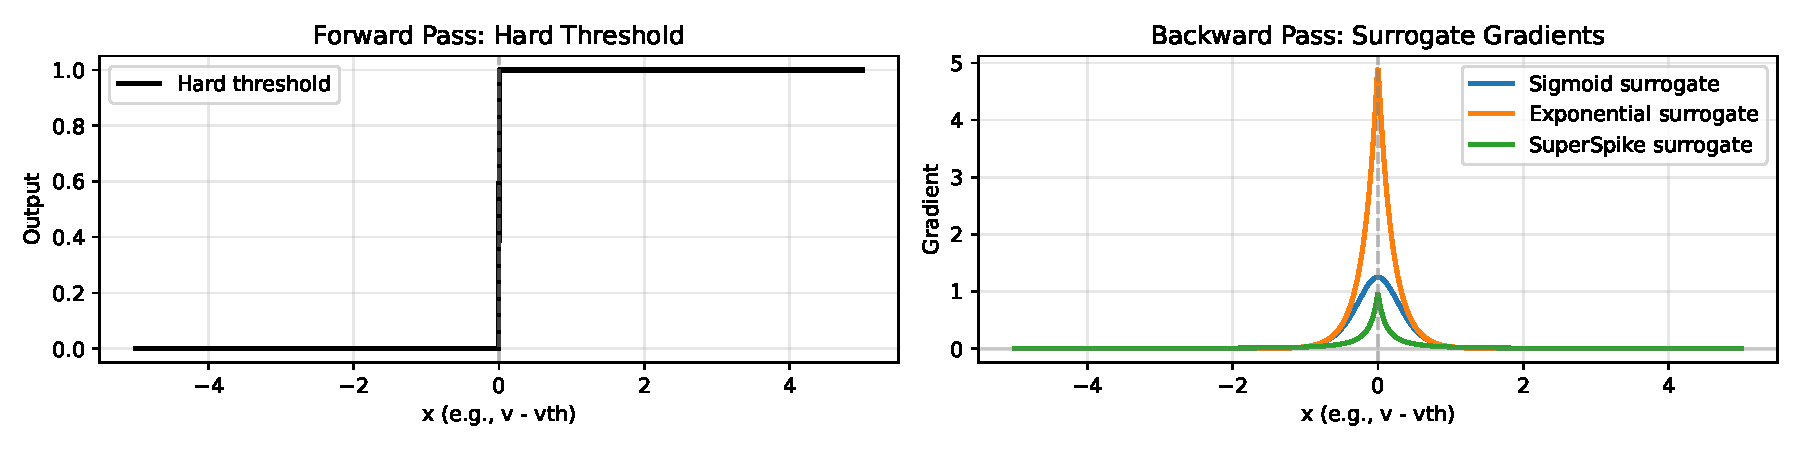
\includegraphics[width=\textwidth]{surrogate_gradients_comparison.pdf}
\end{center}
\end{column}
\end{columns}
\takeaway{Keep the real spike for the forward pass; use a smooth stand-in only for the backward pass.}
\end{frame}

%% ---- SLIDE: But does it work? (transition to depth) ----
\begin{frame}{But does the trick actually work?}
\begin{center}
\begin{tikzpicture}[
    box/.style={draw, rounded corners=6pt, minimum width=5.2cm, minimum height=1.2cm,
                align=center, font=\normalsize, thick}
]
    \node[box, fill=light green] (snn) at (0,1.4) {Deep spiking networks\\[2pt]\small train \emph{thousands of weights}};
    \node[box, fill=light yellow] (us) at (0,-1.4) {A single simplified neuron\\[2pt]\small fit \emph{a handful of parameters}};
    \node[font=\small, right, align=left, text=dark green] at (3.0,1.4) {surrogates\\ work well};
    \node[font=\small, right, align=left, text=dark brick] at (3.0,-1.4) {\textbf{untested}};
    \draw[->, very thick, gray] (snn) -- (us) node[midway, right, font=\small, text=black] {\ does it transfer?};
\end{tikzpicture}
\end{center}
\vspace{0.2cm}
\begin{center}
\large\textbf{Research question:} can surrogate gradients produce useful\\parameter updates for the \hl{AdEx} neuron model?
\end{center}
\takeaway{Sub-questions: which loss makes it work, and where does it fail vs.\ derivative-free search?}
\end{frame}

%% ============================================================
%% PART II -- THE MODEL AND THE MACHINERY
%% ============================================================
\section{The Model and the Machinery}
\insertsectionpage

%% ---- SLIDE: AdEx model ----
\begin{frame}{The AdEx neuron model}
\begin{columns}[T]
\begin{column}{0.58\textwidth}
\textbf{Membrane potential}
\begin{equation*}
  C_m \frac{dV}{dt} = -g_L(V - E_L) + g_L\Delta_T e^{\frac{V-V_T}{\Delta_T}} + I - w
\end{equation*}
\textbf{Adaptation current}
\begin{equation*}
  \tau_w \frac{dw}{dt} = a(V - E_L) - w
\end{equation*}
\textbf{Reset} \quad if $V > 0$\,mV:
\begin{equation*}
  V \rightarrow V_r, \qquad w \rightarrow w + b
\end{equation*}
\end{column}
\begin{column}{0.4\textwidth}
\small
\begin{itemize}
  \item Reproduces \hl{many firing patterns} with \hl{few parameters}.
  \item Some parameters are \emph{physiological} ($C_m$, $g_L$, $E_L$).
  \item Others ($a$, $b$, $\tau_w$) have \bad{no direct counterpart} $\Rightarrow$ must be fitted.
  \item The reset is the \alert{non-differentiable} part.
\end{itemize}
\end{column}
\end{columns}
\takeaway{A favourable accuracy/cost balance --- if we can fit its parameters efficiently.}
\end{frame}

%% ---- SLIDE: Vanishing gradients ----
\begin{frame}{Two gradient problems, not one}
\begin{columns}[c]
\begin{column}{0.46\textwidth}
\small
The surrogate fixes the reset. But differentiating a $\sim$5000-step simulation adds a \bad{second} problem:
\[
\frac{\partial v_{t+1}}{\partial v_t}=\underbrace{(1-H)\tfrac{\partial v^*}{\partial v_t}}_{\text{leak decay}}+\underbrace{(V_r-v^*)\,\varphi_\beta}_{\text{surrogate restores this}}
\]
\begin{itemize}
  \item \good{Fixed:} zero gradient \emph{at} the spike.
  \item \bad{Not fixed:} gradients \alert{decay through leak dynamics} over thousands of steps.
\end{itemize}
\end{column}
\begin{column}{0.53\textwidth}
\begin{center}
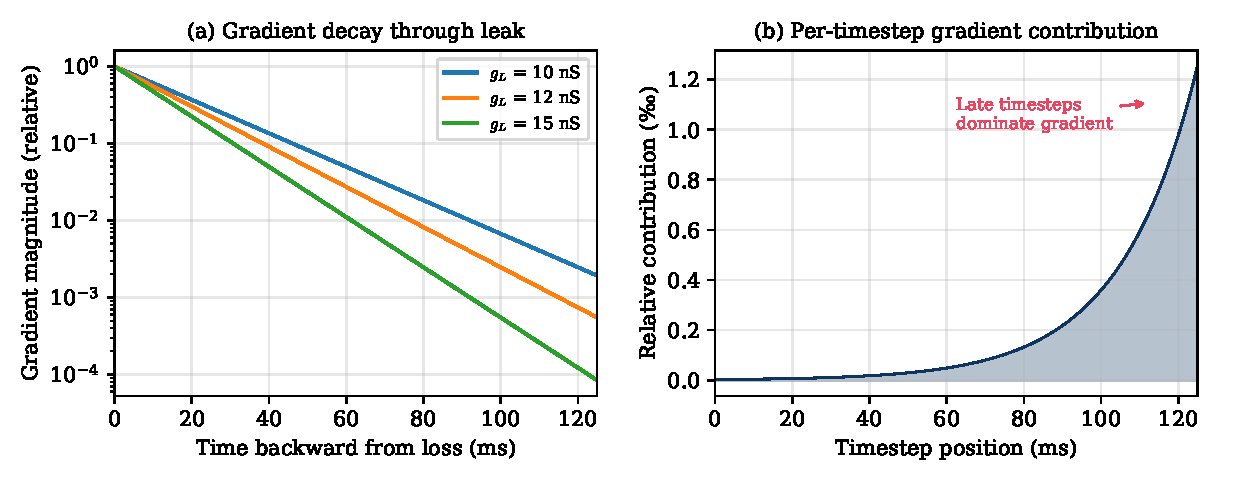
\includegraphics[width=\textwidth]{vanishing-gradients.pdf}
\end{center}
\end{column}
\end{columns}
\takeaway{$b$ and $\tau_w$ are hit hardest: they only act at spikes, then must survive the decay backward.}
\end{frame}

%% ---- SLIDE: surrogate families ----
\begin{frame}{The surrogate is a choice, not a fact}
\begin{columns}[c]
\begin{column}{0.5\textwidth}
\begin{center}
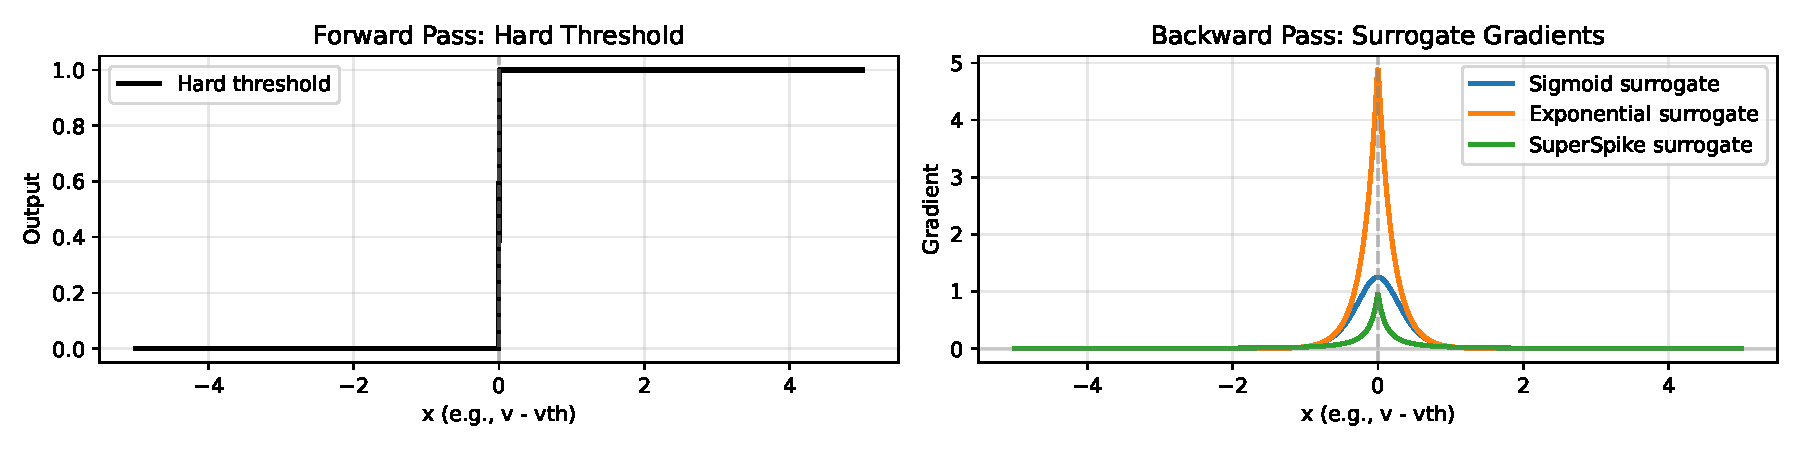
\includegraphics[width=\textwidth]{surrogate_gradients_comparison.pdf}
\end{center}
\end{column}
\begin{column}{0.48\textwidth}
\small
Three common surrogate kernels $\varphi_\beta(x)$, $x = V-V_{\text{th}}$:
\begin{itemize}
  \item \textbf{Sigmoid} --- narrow, exponentially suppressed tails.
  \item \textbf{Exponential} --- intermediate.
  \item \textbf{SuperSpike} --- $1/(\beta|x|+1)^2$, \hl{heavy tails}.
\end{itemize}
\vspace{0.2cm}
Slope $\beta$ sets the width of the ``active window''.
It need not be the true gradient --- only a \emph{useful descent direction}.
\end{column}
\end{columns}
\takeaway{Kernel family and $\beta$ turn out to matter enormously for where gradient signal exists.}
\end{frame}

%% ============================================================
%% PART III -- CONTRIBUTION 1: A DIFFERENTIABLE ADEX
%% ============================================================
\section{Contribution 1: A Differentiable AdEx in Jaxley}
\insertsectionpage

%% ---- SLIDE: implementation ----
\begin{frame}{A differentiable AdEx channel for \texttt{Jaxley}}
\begin{columns}[c]
\begin{column}{0.52\textwidth}
\begin{center}
\begin{tikzpicture}[
    box/.style={draw, rounded corners, minimum width=2.6cm, minimum height=1cm, align=center, font=\small},
    arrow/.style={->, thick, >=stealth}
]
    \node[box, fill=light blue] (jax) at (0,2.5) {JAX\\(autodiff)};
    \node[box, fill=light green] (jaxley) at (0,0) {Jaxley\\(simulator)};
    \node[box, fill=light yellow] (adex) at (4.4,0) {AdEx\\channel};
    \node[box, fill=light brick] (surr) at (4.4,2.5) {Surrogate\\reset};
    \node[box, fill=light turquoise] (opt) at (8.6,1.25) {Gradient\\fitting};
    \draw[arrow] (jax) -- (jaxley);
    \draw[arrow] (jaxley) -- (adex);
    \draw[arrow] (surr) -- (adex);
    \draw[arrow] (jax) -- (surr);
    \draw[arrow] (adex) -- (opt);
    \draw[arrow] (surr) -- (opt);
\end{tikzpicture}
\end{center}
\end{column}
\begin{column}{0.46\textwidth}
\small
\textbf{Continuous reset} enables autodiff:
\[
V_{\text{new}} = s\,V_r + (1-s)\,V,\quad s=H(V-V_{\text{th}})
\]
\begin{itemize}
  \item $s\in\{0,1\}$ in the forward pass --- \emph{identical} dynamics.
  \item \texttt{jax.custom\_vjp} routes $\varphi_\beta$ only on the backward pass.
  \item Same pattern extends to LIF \& Izhikevich.
\end{itemize}
\end{column}
\end{columns}
\takeaway{Contributed upstream to \texttt{Jaxley} (PR \#780) --- the first surrogate-gradient fit path for its simplified models.}
\end{frame}

%% ---- SLIDE: verification ----
\begin{frame}{It is correct: verified against Brian2}
\begin{center}
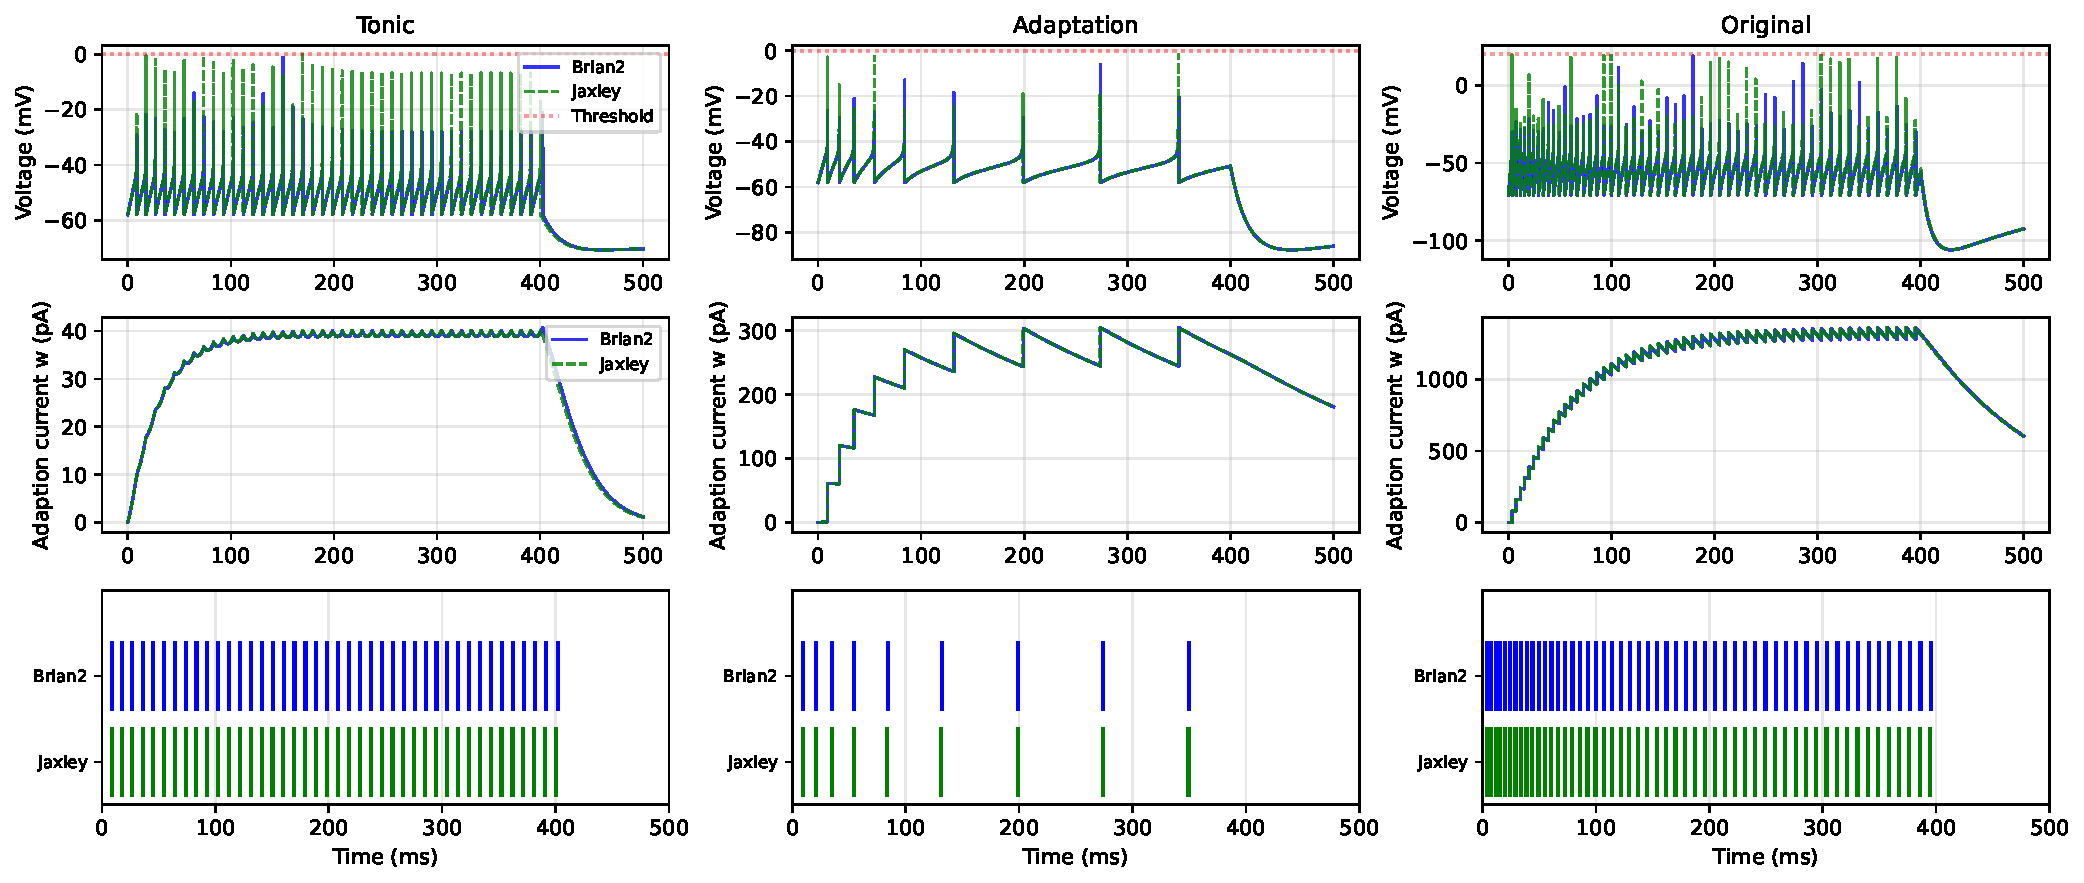
\includegraphics[width=\textwidth,height=0.56\textheight,keepaspectratio]{adex_comparison_combined.pdf}
\end{center}
\begin{center}
\small Three firing regimes (tonic / adaptation / original): \good{identical spike counts}, max spike-timing difference \good{$<1$\,ms}.
\end{center}
\takeaway{The forward model is not the bottleneck --- every later failure is a property of \emph{optimization}, not the dynamics.}
\end{frame}

%% ---- SLIDE: runtime ----
\begin{frame}{It is fast: differentiable \emph{and} competitive}
\begin{columns}[c]
\begin{column}{0.54\textwidth}
\begin{center}
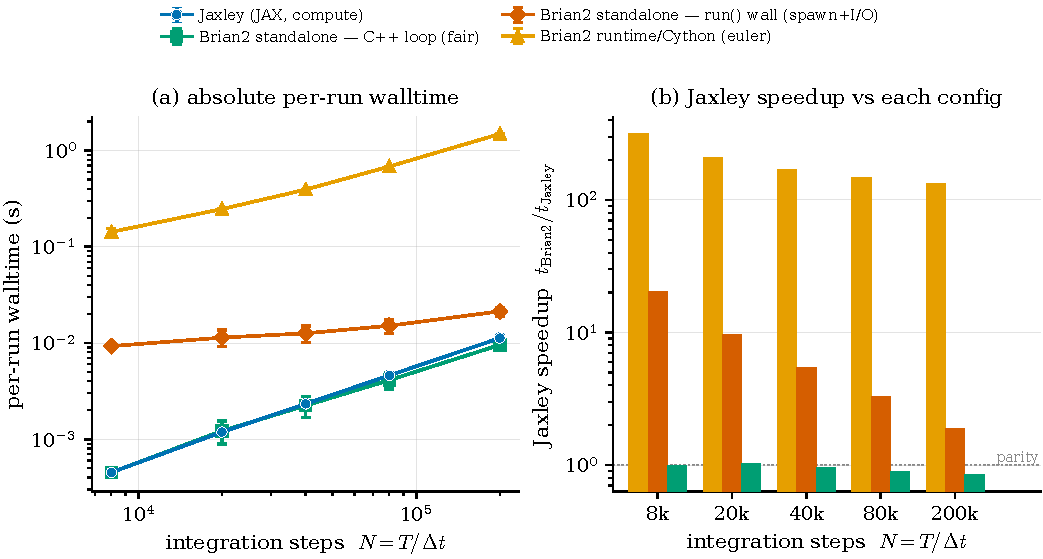
\includegraphics[width=\textwidth]{walltime_standalone_spectrum.pdf}
\end{center}
\end{column}
\begin{column}{0.44\textwidth}
\small
\begin{itemize}
  \item \good{$\sim$200$\times$} faster than Brian2's default runtime mode.
  \item \hl{On par} with hand-optimized, target-compiled C++ (\texttt{cpp\_standalone}).
  \item Stays \textbf{end-to-end differentiable}, \texttt{vmap}-batchable, GPU/TPU-portable --- for free.
\end{itemize}
\end{column}
\end{columns}
\takeaway{Raw throughput of compiled C++, without giving up differentiability or accelerators.}
\end{frame}

%% ============================================================
%% PART IV -- THE CORE QUESTION: LOSS FUNCTIONS
%% ============================================================
\section{The Core Challenge: the Loss Function}
\insertsectionpage

%% ---- SLIDE: gradient tells how, loss tells where ----
\begin{frame}{Gradients tell you \emph{how}; the loss tells you \emph{where}}
\begin{center}
\begin{tikzpicture}[
    box/.style={draw, rounded corners=5pt, minimum width=4.6cm, minimum height=0.95cm,
                align=center, font=\normalsize, thick}
]
    \node[box, fill=light brick] (mse) at (0,2.4) {Pointwise (MSE)};
    \node[font=\small, dark brick, right] at (2.7,2.4) {``suppress all spikes''};
    \node[box, fill=light yellow] (feat) at (0,0.4) {Feature-based};
    \node[font=\small, dark yellow, right] at (2.7,0.4) {right count, brittle timing};
    \node[box, fill=light green] (dist) at (0,-1.6) {Distance-based};
    \node[font=\small, dark green, right] at (2.7,-1.6) {timing-aware spike trains};
    \draw[->, thick] (mse) -- (feat);
    \draw[->, thick] (feat) -- (dist);
\end{tikzpicture}
\end{center}
\vspace{0.1cm}
\begin{center}
\small We compare three differentiable losses --- and the machinery to make discrete spike features differentiable (soft threshold + soft-argmax).
\end{center}
\takeaway{A perfect gradient down a badly-shaped loss still walks off a cliff. Loss design \emph{is} the research problem.}
\end{frame}

%% ---- SLIDE: MSE fails ----
\begin{frame}{Why MSE fails: the non-spiking attractor}
\begin{columns}[c]
\begin{column}{0.55\textwidth}
\begin{center}
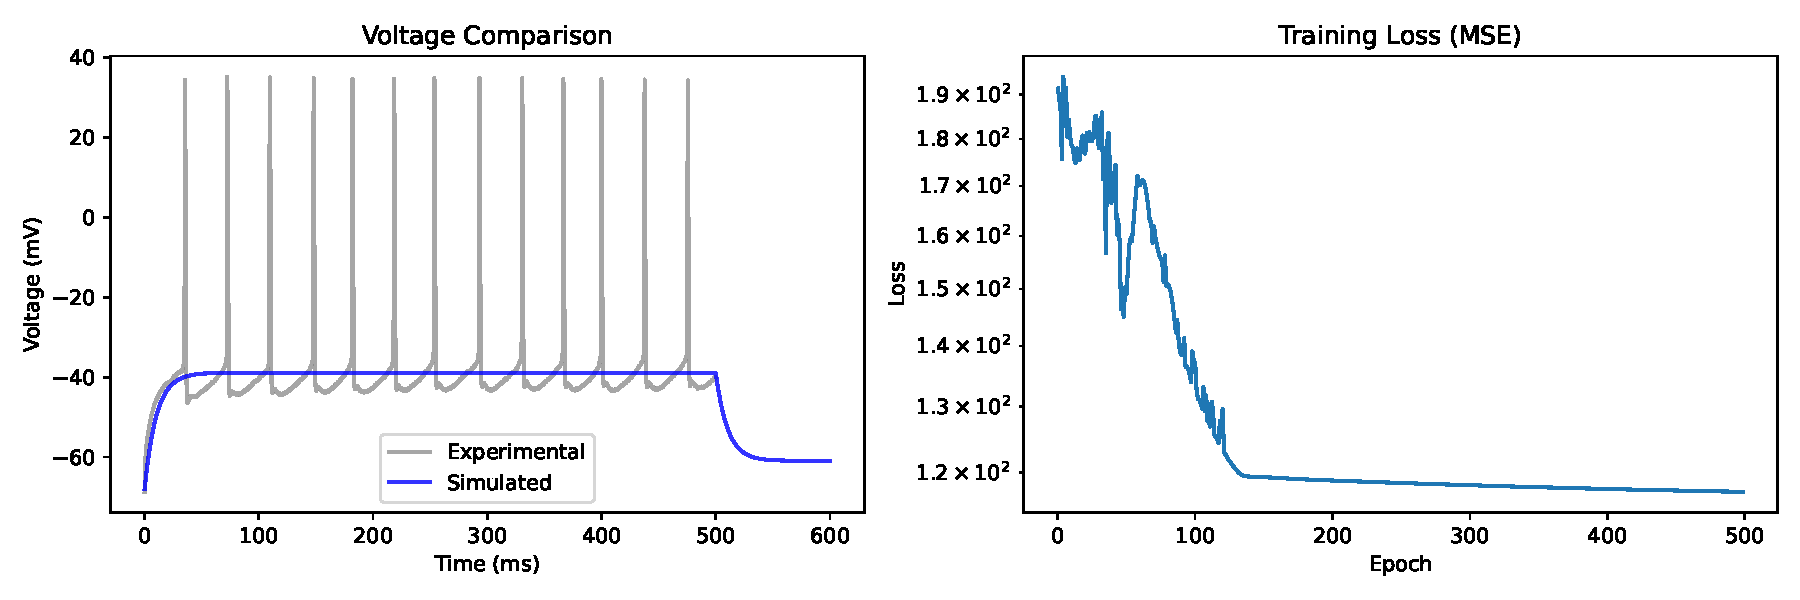
\includegraphics[width=\textwidth]{mse_training_results.pdf}
\end{center}
\end{column}
\begin{column}{0.43\textwidth}
\small
A tiny timing offset makes every spike land on the other trace's \emph{subthreshold} voltage.
\begin{itemize}
  \item Deleting a spike lowers pointwise error \bad{more} than aligning it.
  \item So the optimizer learns to \alert{go silent}.
  \item The loss drops \emph{monotonically} into a genuine minimum.
\end{itemize}
\end{column}
\end{columns}
\takeaway{MSE's gradient points \emph{away} from the spiking solution --- a structural failure, no hyperparameters to blame.}
\end{frame}

%% ---- SLIDE: landscape geometry ----
\begin{frame}{The loss landscape: narrow valleys, wide plateaus}
\begin{columns}[c]
\begin{column}{0.5\textwidth}
\begin{center}
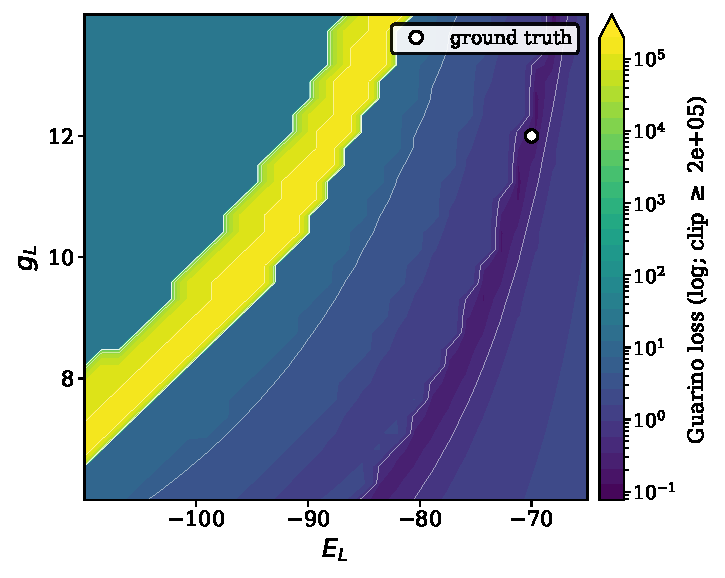
\includegraphics[width=\linewidth,height=0.56\textheight,keepaspectratio]{guarino_focus_E_L_g_L_loss.pdf}
\end{center}
\end{column}
\begin{column}{0.5\textwidth}
\begin{center}
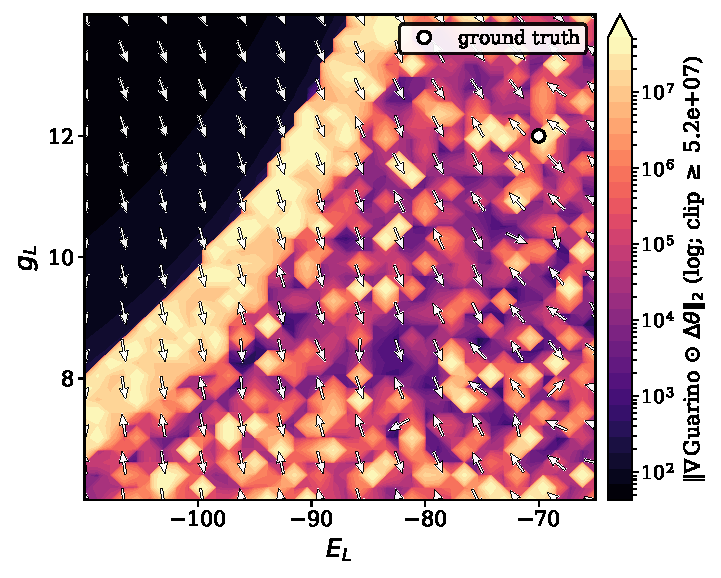
\includegraphics[width=\linewidth,height=0.56\textheight,keepaspectratio]{guarino_focus_E_L_g_L_grad.pdf}
\end{center}
\end{column}
\end{columns}
\begin{center}
\small Guarino loss (left) and gradient field (right) on the $E_L$--$g_L$ plane, log scale.
\end{center}
\takeaway{A thin spiking valley beside a huge silent plateau, whose gradient points \alert{towards a penalty ridge} --- not the valley.}
\end{frame}

%% ---- SLIDE: worked example (it can work) ----
\begin{frame}{It \emph{can} work: a clean recovery}
\begin{columns}[c]
\begin{column}{0.6\textwidth}
\begin{center}
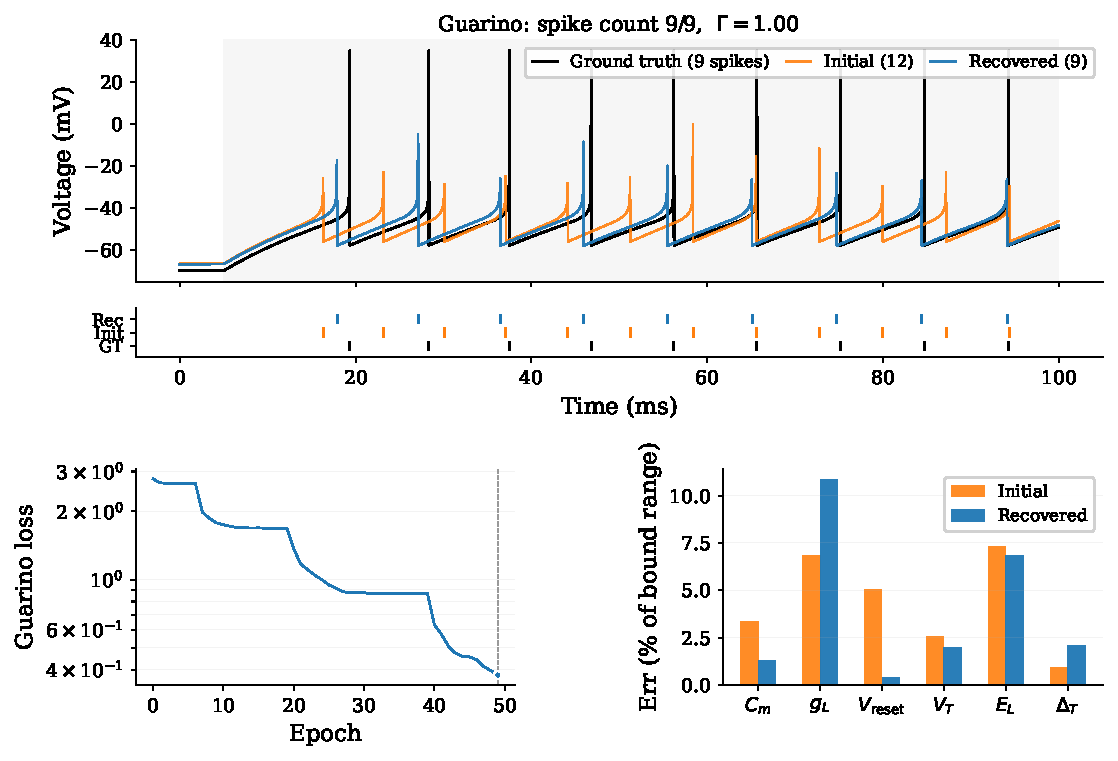
\includegraphics[width=\linewidth,height=0.72\textheight,keepaspectratio]{guarino_synthetic_recovery.pdf}
\end{center}
\end{column}
\begin{column}{0.38\textwidth}
\small
Small ($\sim$15\%) perturbation, six membrane parameters, Guarino loss:
\begin{itemize}
  \item recovered trace matches spike-for-spike, \good{$\Gamma = 1.00$}.
  \item \emph{but} $g_L$ drifts \bad{further} from truth --- parameters trade off along correlated axes.
\end{itemize}
\end{column}
\end{columns}
\takeaway{Viable in principle --- yet already under-constrained. How far does this success region extend?}
\end{frame}

%% ============================================================
%% PART V -- THE HEADLINE RESULT
%% ============================================================
\section{The Verdict: a Systematic Benchmark}
\insertsectionpage

%% ---- SLIDE: benchmark design ----
\begin{frame}{The recovery-radius benchmark}
\begin{columns}[T]
\begin{column}{0.52\textwidth}
\small
\textbf{Setup.} Perturb a known ground truth by $\delta$ in a random direction; try to recover it.
\begin{itemize}
  \item 5 methods $\times$ 3 regimes $\times$ 6 scales $\times$ 30 directions
  \item \good{$= 2{,}700$ paired runs}
  \item success $\equiv$ coincidence factor $\Gamma > 0.5$
\end{itemize}
\end{column}
\begin{column}{0.46\textwidth}
\small
\textbf{Methods, matched on one objective:}
\begin{itemize}
  \item \texttt{grad\_mse}, \texttt{grad\_guarino}, \texttt{grad\_vanrossum}
  \item \texttt{nm\_guarino} --- Nelder--Mead, \emph{same} soft loss
  \item \texttt{nm\_guarino\_hard} --- exact features
\end{itemize}
\vspace{0.2cm}
The only thing that changes between grad and NM is the \hl{gradient consumer}.
\end{column}
\end{columns}
\takeaway{A like-for-like contest: gradient descent vs.\ a derivative-free simplex on the \emph{identical} loss surface.}
\end{frame}

%% ---- SLIDE: headline curves ----
\begin{frame}{The uncomfortable headline}
\begin{center}
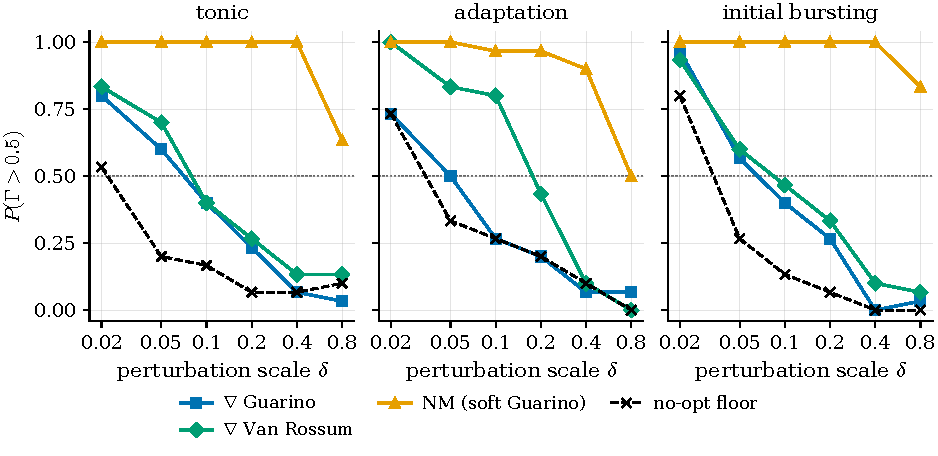
\includegraphics[width=\textwidth,height=0.6\textheight,keepaspectratio]{recovery_radius_curves.pdf}
\end{center}
\begin{center}
\small $P(\Gamma>0.5)$ vs.\ perturbation $\delta$. \bad{Every gradient method} sits at or below the no-optimization floor; \good{both Nelder--Mead variants} dominate everywhere.
\end{center}
\takeaway{Across all 2{,}700 runs, no gradient method matched the simplex on the same objective.}
\end{frame}

%% ---- SLIDE: results table ----
\begin{frame}{Recovery radii: the numbers}
\begin{center}
\small
\begin{tabular}{lcccccc}
\toprule
& \multicolumn{2}{c}{\textbf{tonic}} & \multicolumn{2}{c}{\textbf{adaptation}} & \multicolumn{2}{c}{\textbf{bursting}} \\
\cmidrule(lr){2-3}\cmidrule(lr){4-5}\cmidrule(lr){6-7}
\textbf{Method} & $\delta_{50}$ & $\Gamma_{0.05}$ & $\delta_{50}$ & $\Gamma_{0.05}$ & $\delta_{50}$ & $\Gamma_{0.05}$ \\
\midrule
\texttt{grad\_mse}        & --     & $0.00$ & --     & $0.00$ & --     & $0.00$ \\
\texttt{grad\_guarino}    & $0.02$ & $0.13$ & --     & $0.28$ & $0.02$ & $0.19$ \\
\texttt{grad\_vanrossum}  & --     & $0.07$ & $0.05$ & \hl{$0.62$} & $0.02$ & $0.12$ \\
\texttt{nm\_guarino}      & \good{$0.2$}  & \good{$1.00$} & \good{$0.2$}  & \good{$1.00$} & \good{$0.4$}  & \good{$1.00$} \\
\texttt{nm\_guarino\_hard}& \good{$0.2$}  & \good{$1.00$} & \good{$0.2$}  & \good{$1.00$} & \good{$0.4$}  & \good{$1.00$} \\
\midrule
\texttt{init\_floor}      & $0.02$ & $0.07$ & $0.02$ & $0.32$ & $0.02$ & $0.01$ \\
\bottomrule
\end{tabular}
\end{center}
\vspace{0.15cm}
\small The two NM variants (soft vs.\ exact features) are \emph{indistinguishable} --- the soft approximations don't hurt the simplex. So the difference is the gradient, not the loss.
\takeaway{Gradient fitting works only inside basins already small enough for derivative-free search to cover.}
\end{frame}

%% ---- SLIDE: the revealing exception ----
\begin{frame}{The revealing exception: below threshold}
\begin{columns}[c]
\begin{column}{0.56\textwidth}
\begin{center}
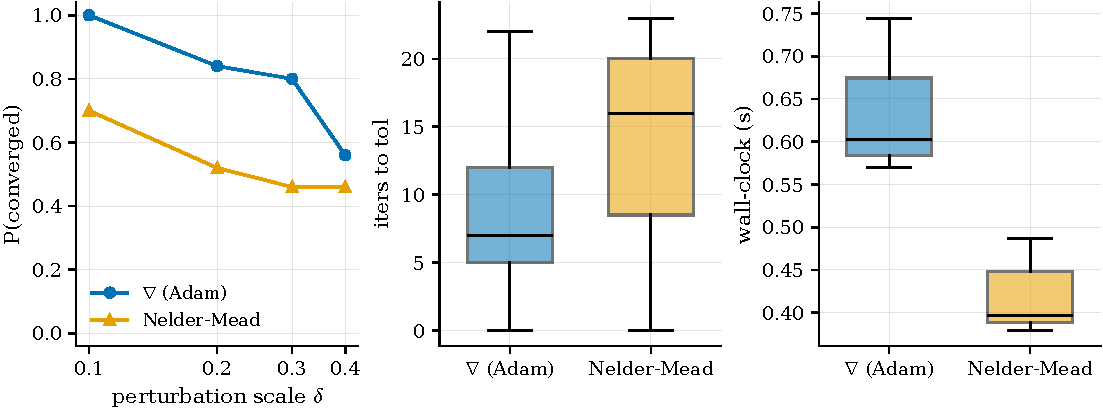
\includegraphics[width=\textwidth]{subthreshold_convergence.pdf}
\end{center}
\end{column}
\begin{column}{0.42\textwidth}
\small
Remove the spikes entirely (fit $\{C_m, E_L, g_L\}$ below rheobase):
\begin{itemize}
  \item gradient descent converges on \good{80\%} vs.\ Nelder--Mead's \bad{53\%}.
  \item wins at \emph{every} $\delta$; more sample-efficient ($9$ fewer evals, median).
\end{itemize}
\hl{The verdict reverses.}
\end{column}
\end{columns}
\takeaway{With no spike in the way, gradient descent is the \emph{stronger} optimizer --- so the spike mechanism is the culprit.}
\end{frame}

%% ---- SLIDE: diagnosis / three failure modes ----
\begin{frame}{Why it fails: three entangled modes}
\begin{columns}[T]
\begin{column}{0.33\textwidth}
\begin{block}{FM1 --- Biased gradient}
\small The surrogate returns the \emph{exact} gradient of a \emph{different}, smoothed loss. Its minimum is offset by order $1/\beta$. Averaged away in SNNs; lands directly on the fitted parameters here.
\end{block}
\end{column}
\begin{column}{0.33\textwidth}
\begin{block}{FM2 --- Loss landscape}
\small Each loss fights descent in its own way (silent attractor, penalty ridge, spike-count jumps). Comes from the \emph{loss}, not the surrogate --- an exact gradient wouldn't help.
\end{block}
\end{column}
\begin{column}{0.33\textwidth}
\begin{block}{FM3 --- Vanishing}
\small Even if FM1/FM2 were fixed, the signal must survive $\sim$5000 multiplicative leak terms backward. Most speculative; acts at every step.
\end{block}
\end{column}
\end{columns}
\vspace{0.2cm}
\small \good{Nelder--Mead} treats the loss as a black box: it steps over the plateaus that stall gradient descent and never meets FM1 or FM3.
\takeaway{The bottleneck is the spike mechanism and the loss geometry it induces --- not gradient descent itself.}
\end{frame}

%% ============================================================
%% PART VI -- CONCLUSIONS
%% ============================================================
\section{Conclusions}
\insertsectionpage

%% ---- SLIDE: key findings ----
\begin{frame}{Key findings}
\small
\begin{columns}[T]
\begin{column}{0.5\textwidth}
\textbf{\good{What worked}}
\begin{itemize}
  \item[\cmark] Differentiable AdEx in \texttt{Jaxley}, contributed upstream
  \item[\cmark] $\sim$200$\times$ over default Brian2; on par with C++
  \item[\cmark] Surrogate restores gradient flow through spikes
  \item[\cmark] Below threshold, gradient descent \emph{beats} Nelder--Mead
\end{itemize}
\end{column}
\begin{column}{0.5\textwidth}
\textbf{\bad{What did not}}
\begin{itemize}
  \item[\xmark] No gradient method matched Nelder--Mead over 2{,}700 spiking runs
  \item[\xmark] MSE fails structurally (goes silent)
  \item[\xmark] Feature losses: brittle, many hyperparameters
  \item[\xmark] $a$, $b$, $\tau_w$ not recoverable from a single trace
\end{itemize}
\end{column}
\end{columns}
\vspace{0.2cm}
\begin{block}{Main insight}
\centering
The challenge is the \alert{spike mechanism and loss geometry}, not the optimizer.\\ Surrogate success in deep SNNs does \emph{not} transfer automatically to biophysical fitting.
\end{block}
\end{frame}

%% ---- SLIDE: future work ----
\begin{frame}{Where to go from here}
\begin{columns}[T]
\begin{column}{0.5\textwidth}
\textbf{Change the model}
\begin{itemize}
  \item Neuron families with a \hl{closed-form between-spike solution} (QIF / pseudospikes, Klos--Memmesheimer).
  \item Descend the \emph{true} loss, not a smoothed surrogate --- removing FM1 by construction.
\end{itemize}
\end{column}
\begin{column}{0.5\textwidth}
\textbf{Change the loss / signal}
\begin{itemize}
  \item Multi-trace constraints (identifiability).
  \item Hybrid \& signal-processing spike-train distances.
  \item Forward-mode sensitivities \& per-parameter preconditioning to fight FM3.
\end{itemize}
\end{column}
\end{columns}
\vspace{0.2cm}
\small The infrastructure stands regardless: the same fast, batchable simulator also powers derivative-free and simulation-based pipelines.
\takeaway{If exact spike times matter, a different neuron model beats more surrogate tuning on AdEx.}
\end{frame}

%% ---- SLIDE: closing takeaway ----
\begin{frame}{Between two worlds}
\vspace{0.3cm}
\begin{columns}[c]
\begin{column}{0.62\textwidth}
\large
A negative result, precisely bounded:
\vspace{0.3cm}
\begin{itemize}
  \item A \good{fast, differentiable} simplified neuron --- delivered and contributed.
  \item Gradient fitting of spiking AdEx \bad{does not beat} derivative-free search \dots
  \item \dots\ \good{yet} it wins the moment the spike is removed.
\end{itemize}
\end{column}
\begin{column}{0.36\textwidth}
\centering
\hl{\Large Where it fails,\\[4pt] and where\\[4pt] it does not.}
\end{column}
\end{columns}
\vspace{0.4cm}
\centering
\normalsize Thank you --- questions welcome.
\end{frame}

%% ============================================================
%% APPENDIX
%% ============================================================
\appendix
\section{Appendix}
\insertsectionpage

\begin{frame}{Appendix: contents}
\small
\begin{multicols}{2}
\begin{itemize}
  \item[A1] AdEx parameters
  \item[A2] Surrogate kernels (math)
  \item[A3] Coincidence factor $\Gamma$
  \item[A4] Benchmark configuration
  \item[A5] Backprop-through-time
  \item[A6] Gradient existence check
  \item[A7] Feature (Guarino) loss
  \item[A8] Van Rossum \& soft-DTW
  \item[A9] Loss-landscape grids
  \item[A10] Parameter-sensitivity asymmetry
  \item[A11] Van Rossum landscape
  \item[A12] Subthreshold identifiability
  \item[A13] Training stabilization
  \item[A14] Point-neuron geometry bridge
  \item[A15] Runtime detail
  \item[A16] Dataset \& compute
\end{itemize}
\end{multicols}
\end{frame}

%% A1
\begin{frame}{A1: AdEx parameters}
\centering\small
\begin{tabular}{lllc}
\toprule
\textbf{Parameter} & \textbf{Symbol} & \textbf{Default / unit} & \textbf{Trainable} \\
\midrule
Membrane capacitance     & $C_m$        & 200 pF   & Yes \\
Leak conductance         & $g_L$        & 10 nS    & Yes \\
Leak reversal            & $E_L$        & $-70$ mV & Yes \\
Threshold potential      & $V_T$        & $-50$ mV & Yes \\
Slope factor             & $\Delta_T$   & 2 mV     & Yes \\
Reset potential          & $V_r$        & $-58$ mV & Yes \\
Detection threshold      & $v_{\text{th}}$ & 0 mV  & No \\
Adaptation time const.   & $\tau_w$     & 30 ms    & (Yes) \\
Subthreshold adaptation  & $a$          & 2 nS     & (Yes) \\
Spike-triggered adapt.   & $b$          & 0 pA     & (Yes) \\
\bottomrule
\end{tabular}
\vspace{0.3cm}

\footnotesize The six membrane parameters are trainable in the benchmark; $a,b,\tau_w$ are held at ground truth (too weak/noisy a signal from a single trace).
\end{frame}

%% A2
\begin{frame}{A2: Surrogate kernels}
\textbf{Sigmoid}
\[ \varphi_\beta(x) = \beta\,\sigma(\beta x)\,(1-\sigma(\beta x)) \]
\textbf{Exponential}
\[ \varphi_\beta(x) = \beta\,\exp(-\beta|x|) \]
\textbf{SuperSpike}
\[ \varphi_\beta(x) = \frac{1}{(\beta|x|+1)^2} \]
\vspace{0.2cm}
\small $x = V - V_{\text{th}}$; $\beta$ controls the width of the active window. SuperSpike's heavy tail keeps a usable gradient far from threshold; the sigmoid collapses to numerical noise off-threshold at large $\beta$ (down to $10^{-27}$ --- below float32).
\end{frame}

%% A3
\begin{frame}{A3: Coincidence factor $\Gamma$}
\[
\Gamma = \frac{N_{\text{coinc}} - \langle N_{\text{coinc}}\rangle}{\tfrac{1}{2}(N_{\text{data}}+N_{\text{model}})}\cdot\frac{1}{1-2f\Delta}
\]
\begin{itemize}
  \item $N_{\text{coinc}}$: spikes matched within $\pm\Delta = 2$\,ms
  \item $\langle N_{\text{coinc}}\rangle$: expected for a Poisson process of rate $f$
  \item $\Gamma = 1$ perfect; $\Gamma = 0$ chance; $\Gamma < 0$ worse than chance
\end{itemize}
\vspace{0.2cm}
\small Success threshold $\Gamma > 0.5$. Synthetic targets $\Rightarrow$ ceiling is $\Gamma=1$; state-of-the-art on real recordings is $\Gamma\approx 0.82$ (Jolivet et al.).
\end{frame}

%% A4
\begin{frame}{A4: Benchmark configuration}
\centering\footnotesize
\begin{tabular}{lcc}
\toprule
 & \textbf{gradient methods} & \textbf{Nelder--Mead} \\
\midrule
Optimizer          & Polyak SGD & Nelder--Mead \\
Learning rate      & $0.001$ & --- \\
Polyak $(\alpha,\beta)$ & $(0.8,\,0.6)$ & --- \\
Budget             & 25 grad steps & 50 evals \\
Param transform    & sigmoid & box-bounded \\
Surrogate          & SuperSpike, $\beta=6.0$ & not consumed \\
\midrule
Feature temp.\ $\tau$ & $0.3$ & $0.3$ / hard \\
Sigmoid sharpness $\beta$ & $10.0$ & $10.0$ / hard \\
Van Rossum kernel $\tau$ & $8$\,ms & --- \\
\midrule
$\Delta t$         & \multicolumn{2}{c}{$0.025$\,ms} \\
Duration           & \multicolumn{2}{c}{100\,ms (90\,ms stim)} \\
\bottomrule
\end{tabular}
\vspace{0.25cm}

\footnotesize Three gradient losses share optimizer, surrogate and transform --- they differ only in the loss.
\end{frame}

%% A5
\begin{frame}{A5: Backpropagation through time}
The simulation is a recurrence $s_0 \to s_1 \to \dots \to s_T$, $s_t=(V_t,w_t)$:
\[
\frac{\partial L}{\partial\theta}=\sum_{t=0}^{T}\frac{dL}{ds_t}\cdot\frac{\partial s_t}{\partial\theta},\qquad
\frac{dL}{ds_t}=\frac{\partial L}{\partial s_t}+\Big(\frac{\partial s_{t+1}}{\partial s_t}\Big)^{\!\mathsf{T}}\frac{dL}{ds_{t+1}}
\]
\small
The error at time $t$ carries a product of $T-t$ Jacobians. In the subthreshold regime this is dominated by the leak, whose spectral radius $<1$ $\Rightarrow$ exponential decay. The surrogate restores the \emph{spike} term $(V_r-v^*)\varphi_\beta$ but cannot touch the leak decay.
\end{frame}

%% A6
\begin{frame}{A6: Gradient-existence check}
\centering\small
Toy loss $\Loss=-\sum_t s(t)$ (negative spike count), $\partial\Loss/\partial v_{\text{th}}$ on the tonic set:
\vspace{0.2cm}

\begin{tabular}{lr}
\toprule
Channel & $\partial\Loss/\partial v_{\text{th}}$ \\
\midrule
\texttt{AdEx} (hard threshold)        & $0$ exactly \\
\texttt{AdExSurrogate}, sigmoid ($\beta{=}10$)    & $+1.9\times10^{-21}$ \\
\texttt{AdExSurrogate}, exponential ($\beta{=}5$) & $+4.5\times10^{-4}$ \\
\texttt{AdExSurrogate}, SuperSpike ($\beta{=}10$) & $+1.3\times10^{-1}$ \\
\bottomrule
\end{tabular}
\vspace{0.3cm}

\footnotesize The hard channel returns a structural zero; all surrogates give a finite gradient of the correct sign --- but magnitudes span \emph{20 orders of magnitude} at a fixed operating point. Motivates SuperSpike for the benchmark.
\end{frame}

%% A7
\begin{frame}{A7: Feature-based (Guarino) loss}
\[
\Loss_{\text{Guarino}}=\sum_i w_i\cdot\frac{|f_i^{\text{sim}}-f_i^{\text{exp}}|}{|f_i^{\text{exp}}|+\epsilon}
\]
\small
Eight features: $t_1,t_2,t_3,t_{\text{last}}$, $1/\text{ISI}_1$, $1/\text{ISI}_{\text{last}}$, firing rate, $V_{\text{stimend}}$. Plus a fixed penalty per missing feature.
\vspace{0.2cm}

\textbf{Made differentiable} without softening the spike train ($s(t)$ stays binary):
\begin{itemize}
  \item hard threshold ``did a spike occur?'' $\to$ sigmoid gate
  \item hard $\arg\max$ ``which step?'' $\to$ temperature-weighted average (soft-argmax)
\end{itemize}
Gradient enters only through the \texttt{custom\_vjp} on $s(t)$. Cost: four softness hyperparameters, tuned per cell.
\end{frame}

%% A8
\begin{frame}{A8: Van Rossum \& soft-DTW}
\textbf{Van Rossum} --- convolve spike trains with $K(t)=e^{-t/\tau}$, take $L^2$:
\[
\Loss_{\text{VR}}^2=\frac{1}{\tau}\int_0^T\big(f_{\text{sim}}(t)-f_{\text{exp}}(t)\big)^2 dt
\]
\small Naturally differentiable --- surrogate is its \emph{only} bias source. $\tau$: small $=$ timing, large $=$ rate. Optional subthreshold MAE term supplies gradient on the silent plateau.
\vspace{0.2cm}

\textbf{Soft-DTW} --- replace DTW's hard $\min$ with softmin $-\gamma\log\sum e^{-a_i/\gamma}$.
\small Tolerant of temporal shifts, but $O(nm)$, and its landscape has thin deep valleys $\Rightarrow$ recovers only tiny perturbations. Excluded from the method comparison.
\end{frame}

%% A9
\begin{frame}{A9: Loss-landscape grids}
\begin{columns}[c]
\begin{column}{0.34\textwidth}
\centering\scriptsize MSE\\
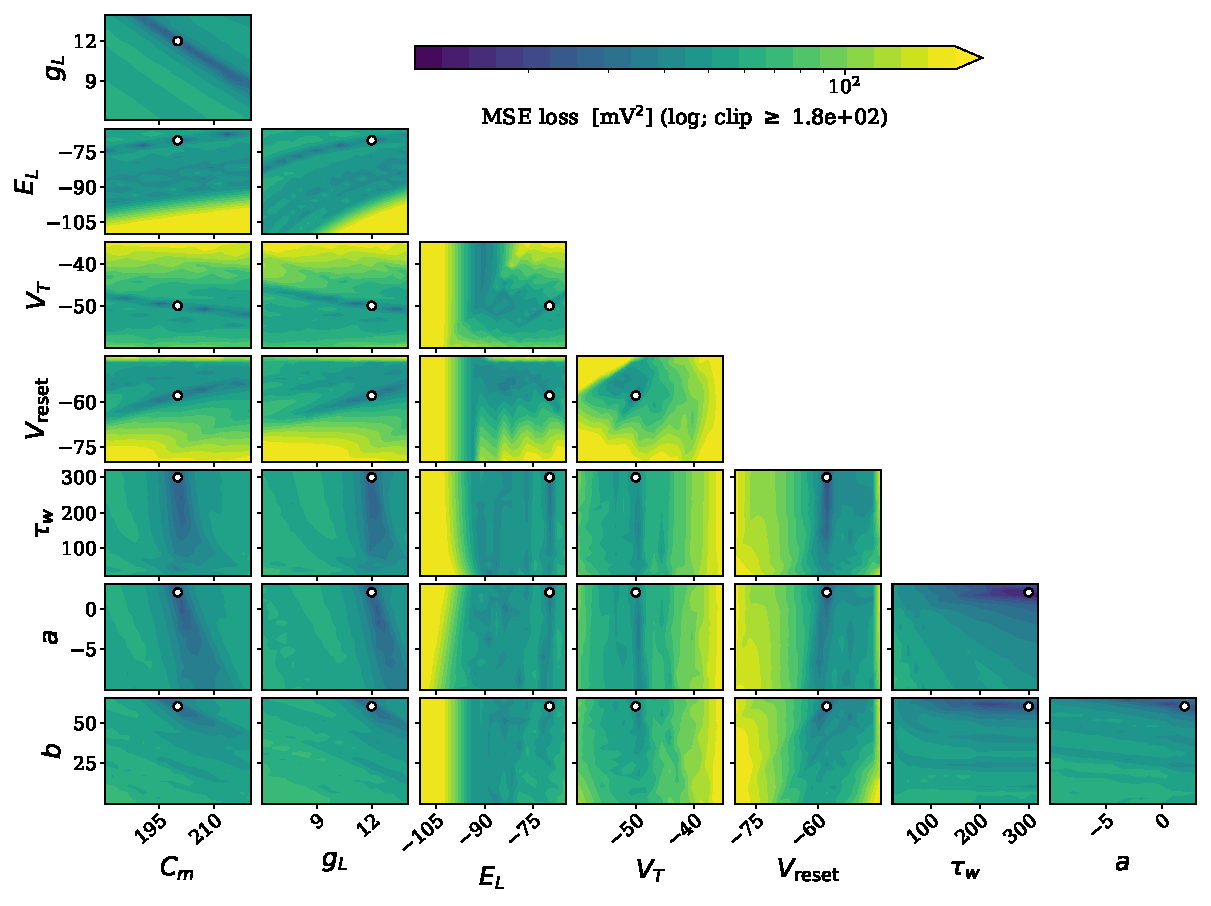
\includegraphics[width=\textwidth]{mse_loss_landscape_grid.pdf}
\end{column}
\begin{column}{0.34\textwidth}
\centering\scriptsize Van Rossum\\
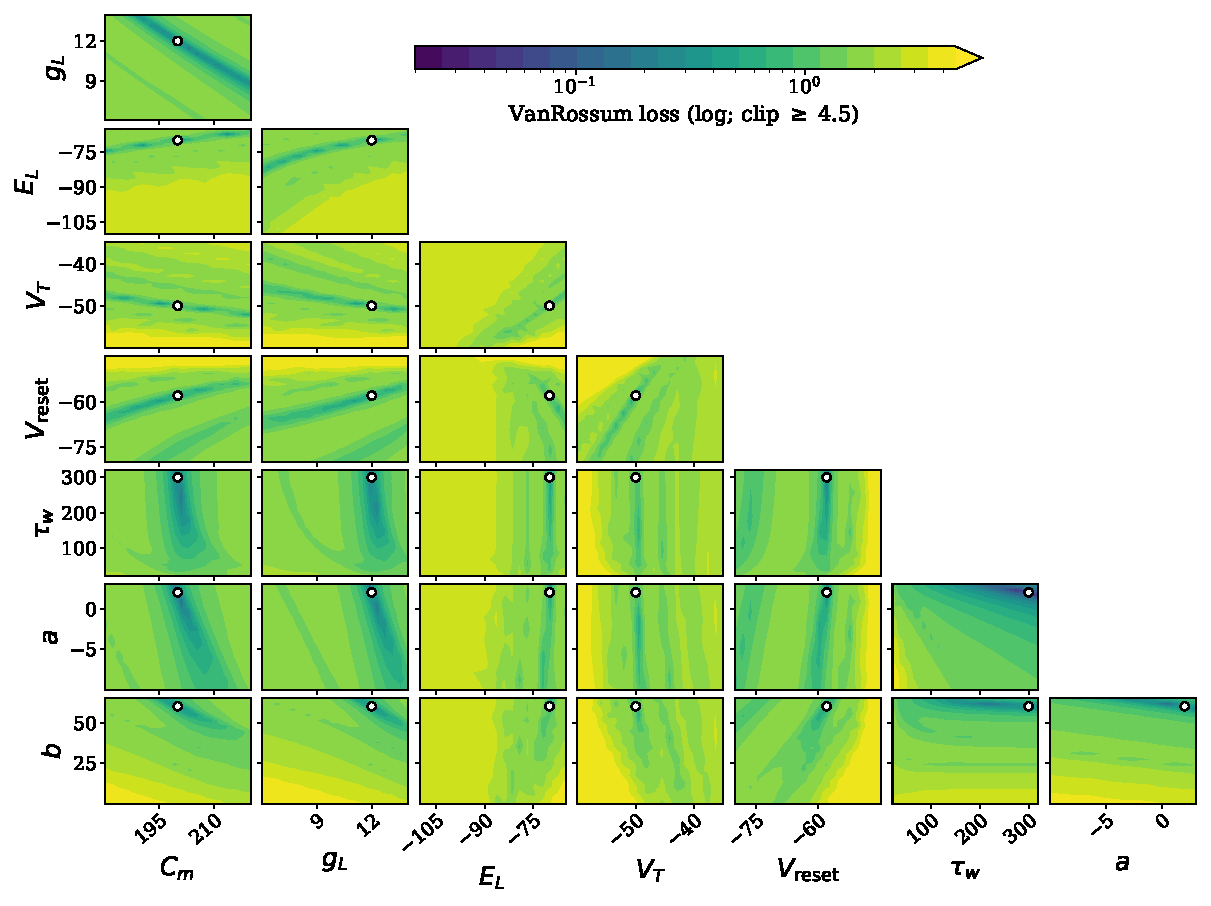
\includegraphics[width=\textwidth]{vanrossum_loss_landscape_grid.pdf}
\end{column}
\begin{column}{0.34\textwidth}
\centering\scriptsize soft-DTW\\
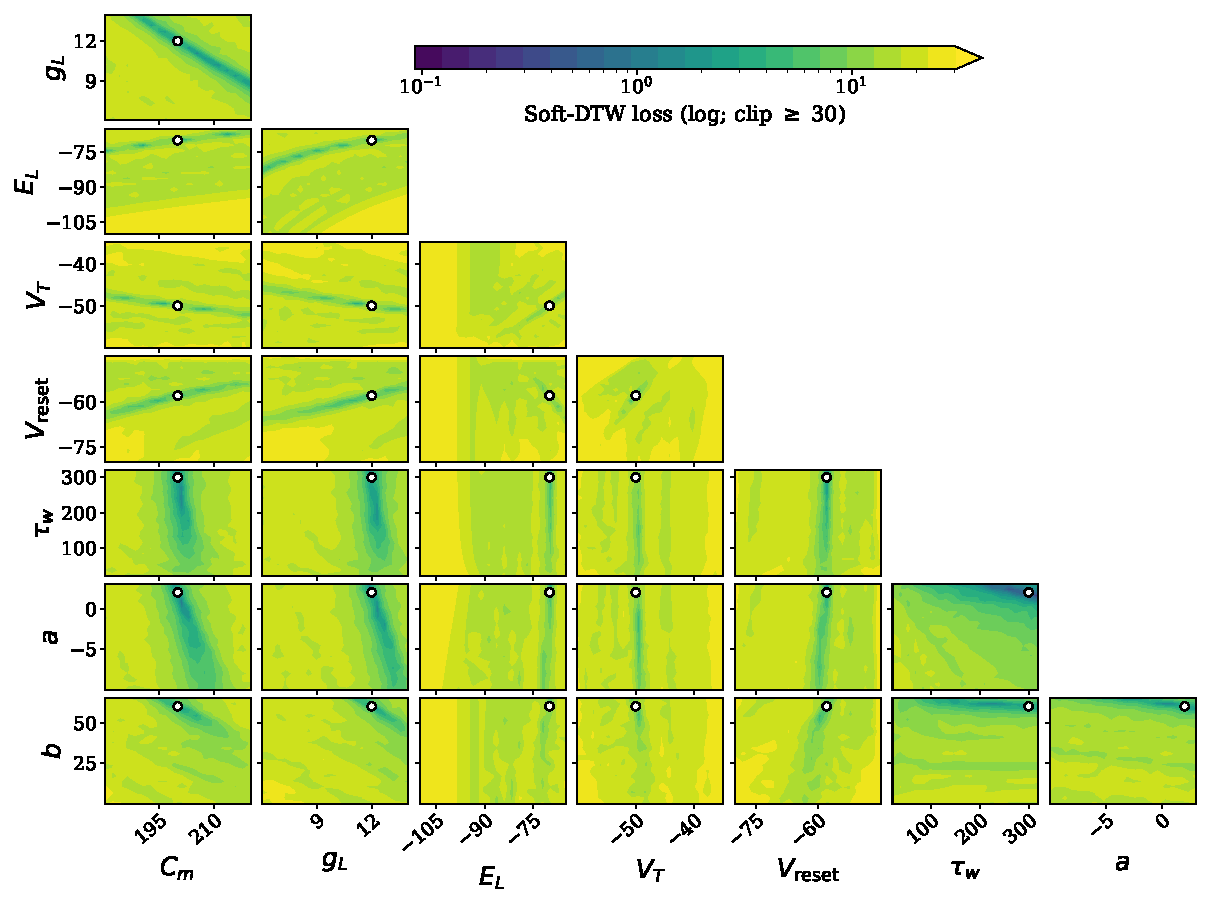
\includegraphics[width=\textwidth]{soft-dtw_loss_landscape_grid.pdf}
\end{column}
\end{columns}
\vspace{0.2cm}
\footnotesize Shared structure across all losses: thin, axis-aligned spiking valleys; large silent plateaus; plateau gradients whose \emph{direction} is not constrained by distance to the valley. MSE has the most local minima; soft-DTW the narrowest valleys.
\end{frame}

%% A10
\begin{frame}{A10: Not all parameters are equal}
\begin{columns}[c]
\begin{column}{0.5\textwidth}
\begin{center}
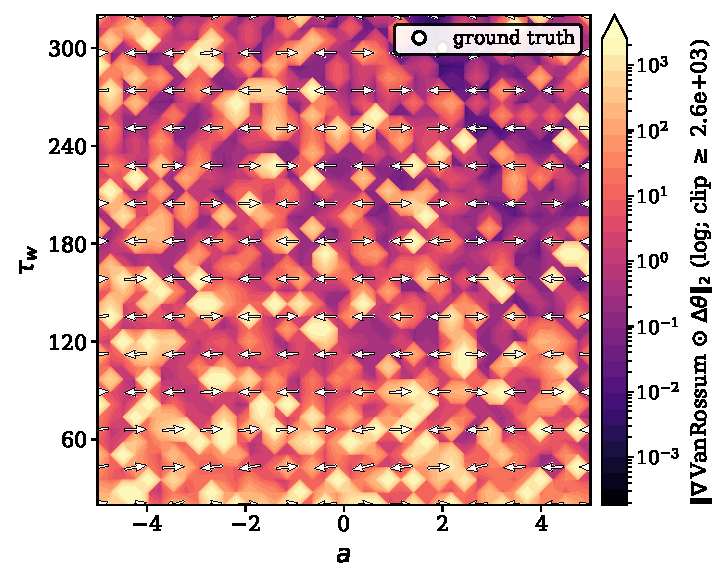
\includegraphics[width=\linewidth,height=0.66\textheight,keepaspectratio]{loss_landscape_focus_vanrossum_a_tau_w_grad2d_superspike_10.pdf}
\end{center}
\end{column}
\begin{column}{0.5\textwidth}
\small
Gradient field on $(a,\tau_w)$ --- dominated by the $a$ component everywhere, even after bound-normalization.
\begin{itemize}
  \item \hl{Continuous} params ($E_L,g_L,C_m,V_T,a$) act every timestep.
  \item \bad{Event-driven} $b$ (spike kicks only) and \bad{slow} $\tau_w$ get almost no signal.
\end{itemize}
\end{column}
\end{columns}
\vspace{0.1cm}
\footnotesize Rescaling units cannot make $b$ act outside spikes --- a structural reason $b,\tau_w$ resist recovery.
\end{frame}

%% A11
\begin{frame}{A11: Van Rossum landscape}
\begin{columns}[c]
\begin{column}{0.5\textwidth}
\begin{center}
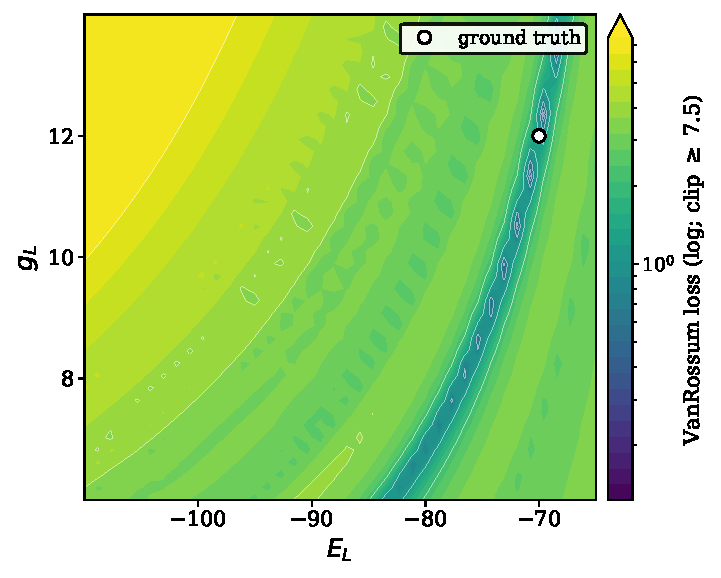
\includegraphics[width=\linewidth,height=0.56\textheight,keepaspectratio]{vanrossum_focus_E_L_g_L_loss.pdf}
\end{center}
\end{column}
\begin{column}{0.5\textwidth}
\begin{center}
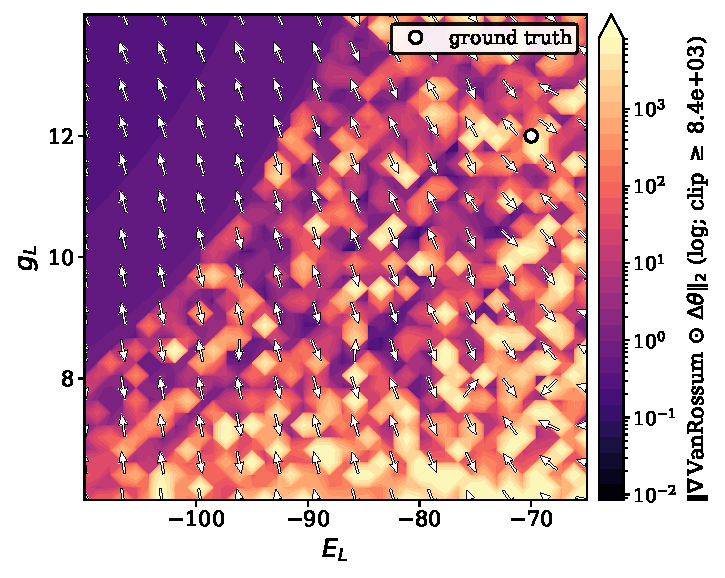
\includegraphics[width=\linewidth,height=0.56\textheight,keepaspectratio]{vanrossum_focus_E_L_g_L_grad.pdf}
\end{center}
\end{column}
\end{columns}
\footnotesize No penalty ridge (unlike Guarino): the loss climbs smoothly to the plateau. But the spiking region shows an order-of-magnitude \emph{checkerboard}: a single grid step adds/removes a spike, and the kernel convolution smooths timing of \emph{existing} spikes, not spike-count changes. Plateau gradient is small ($\sim 10^{-1}$) --- a magnitude bottleneck.
\end{frame}

%% A12
\begin{frame}{A12: Subthreshold identifiability}
\begin{columns}[c]
\begin{column}{0.55\textwidth}
\begin{center}
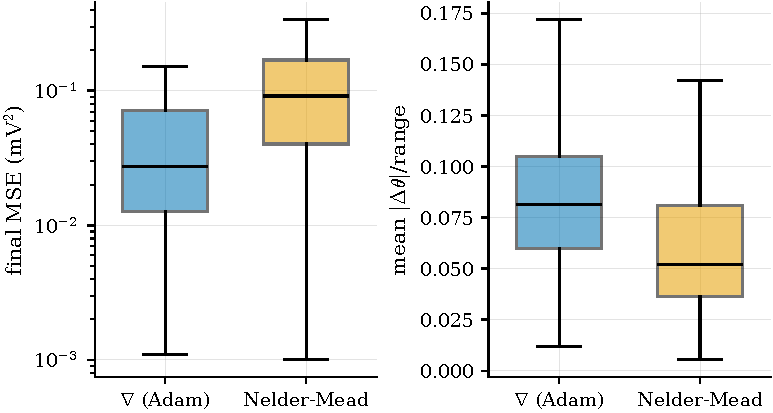
\includegraphics[width=\textwidth]{subthreshold_fit_quality.pdf}
\end{center}
\end{column}
\begin{column}{0.43\textwidth}
\small
Gradient descent reaches \good{lower loss} \dots\ but \bad{not better parameters}.
\begin{itemize}
  \item $C_m,E_L,g_L$ trade off along an extended valley.
  \item Many triples give near-identical traces.
\end{itemize}
A ceiling on \emph{any} single-trace method --- motivates multi-trace fitting.
\end{column}
\end{columns}
\end{frame}

%% A13
\begin{frame}{A13: Training stabilization}
\small
\textbf{Polyak step size} --- $\theta_{t+1}=\theta_t-\eta\frac{|\Loss|^\alpha}{\|\nabla\Loss\|^\beta+\epsilon}\nabla\Loss$: automatic annealing, soft-caps gradient spikes. \emph{Temporal} smoothing only --- does not fix per-parameter magnitude gaps.
\vspace{0.2cm}

\textbf{Sigmoid parameter transform} --- $\theta=\theta_{\min}+(\theta_{\max}-\theta_{\min})\sigma(\tilde\theta)$: bounds enforced implicitly, finite gradient at the boundary (vs.\ hard projection discarding the step). Side effect: hidden bias toward interval centres; sensitive to bound choice.
\vspace{0.2cm}

\textbf{Why they can't rescue it:} the toolbox only rescales gradient \emph{magnitude}. The pathologies that matter are about \alert{direction and existence} --- which rescaling cannot reach.
\end{frame}

%% A14
\begin{frame}{A14: Point-neuron geometry bridge}
\small
AdEx is a point neuron in absolute units (pF, nS, pA). \texttt{Jaxley} is geometry-aware (densities, surface areas). We bridge with a \emph{fixed fictitious} cylinder, $A = 100\,\mu\text{m}^2$:
\begin{itemize}
  \item all dynamics computed in \texttt{update\_states} (\texttt{compute\_current}$=0$) $\Rightarrow$ no double integration;
  \item current conversion collapses to $I_{\text{nA}} = I_{\text{pA}}/1000$ (numerically);
  \item geometry fixed $\Rightarrow$ \textbf{$C_m$ stays trainable} with no geometry recompute.
\end{itemize}
\vspace{0.15cm}
\footnotesize Lets a simplified point neuron live cleanly inside an HH-oriented compartmental simulator.
\end{frame}

%% A15
\begin{frame}{A15: Runtime detail}
\centering\small
\begin{tabular}{rrrrr}
\toprule
$T$ (ms) & steps & Jaxley (ms) & Brian2 (ms) & speedup \\
\midrule
200  & 8\,000   & 0.462  & 142.53  & 308$\times$ \\
500  & 20\,000  & 1.129  & 246.64  & 218$\times$ \\
1000 & 40\,000  & 2.269  & 393.18  & 173$\times$ \\
2000 & 80\,000  & 4.540  & 682.87  & 150$\times$ \\
5000 & 200\,000 & 11.251 & 1489.74 & 132$\times$ \\
\bottomrule
\end{tabular}
\vspace{0.25cm}

\footnotesize vs.\ Brian2 \emph{default} runtime (geo-mean $188\times$). vs.\ best-case compiled \texttt{cpp\_standalone} the compute-vs-compute comparison is a tie ($1.0\times$--$0.9\times$). The point is not out-computing a C compiler --- it is matching it \emph{while staying differentiable and GPU-portable}. Per-step: $0.056\,\mu$s (Jaxley) vs.\ $6.96\,\mu$s (Brian2).
\end{frame}

%% A16
\begin{frame}{A16: Dataset \& compute}
\small
\textbf{Recordings.} Striatal projection neurons, Johansson \& Silberberg (2020), cleaned by Kozlov et al. (2025). Intracellular current-clamp. Benchmark uses \emph{synthetic} targets (same model family) so recovery is measurable in isolation.
\vspace{0.2cm}

\textbf{Compute.} Everything on a single Apple MacBook Air (M1), JAX on CPU for reproducibility. Gradient run $\sim$1\,s; Nelder--Mead $\sim$5--10\,s. Full 2{,}700-run benchmark $\approx$ 2\,h.
\vspace{0.2cm}

\textbf{Files.} voltage \texttt{*\_ch5\_*.dat}, current \texttt{*\_ch4\_*.dat} (mV, pA, ms).
\end{frame}

\insertendpage

\end{document}
